\documentclass[xcolor={table,dvipsnames}]{beamer}
\usetheme{UASLP1}

\usepackage[utf8]{inputenc}
\usepackage[T1]{fontenc}
\usepackage[spanish]{babel}
\usepackage{longtable}
\usepackage{array}
\usepackage{booktabs}
\usepackage{tabularx}
%% Fuente
\usepackage{helvet}
\usepackage[numbers]{natbib}
\bibliographystyle{ieeetr}
\usepackage{subcaption}
\usepackage{graphicx}
\usepackage{listings}
\definecolor{codegray}{rgb}{0.5,0.5,0.5}
\definecolor{codepurple}{rgb}{0.58,0,0.82}
\definecolor{backcolour}{rgb}{0.95,0.95,0.95}
\definecolor{codeblue}{rgb}{0.1,0.1,0.7}

\addto\captionsspanish{\renewcommand{\tablename}{Tabla}}
\addto\captionsspanish{\renewcommand{\listtablename}{Indice de tablas}}

\lstdefinestyle{pythonstyle}{
    language=Python,
    backgroundcolor=\color{backcolour},
    commentstyle=\color{codegray}\itshape,
    keywordstyle=\color{codeblue}\bfseries,
    stringstyle=\color{codepurple},
    basicstyle=\ttfamily\scriptsize,
    numbers=left,
    numberstyle=\tiny\color{codegray},
    stepnumber=1,
    numbersep=5pt,
    showspaces=false,
    showstringspaces=false,
    showtabs=false,
    frame=single,
    breaklines=true,
    breakatwhitespace=true,
    tabsize=4,
    captionpos=b
}

\title{\large{DISE\~NO Y CONSTRUCCI\'ON DE UN EXOESQUELETO OPTIMIZANDO LOS MECANISMOS PARA AGARRE DE PINZA FINA}}

\author{
\textbf{Ing. Adriana Elorza Ramos} \\
\textbf{Director: Dr. Manuel Arias Montiel} \\
\textbf{Co-directora: Dra. Esther Lugo Gonz\'alez}
}

\date{\today}

\AtBeginSection[]{
\begin{frame}{Indice}
\tableofcontents[currentsection]
\end{frame}
}

\begin{document}

%---------------- Portada ----------------%
\begin{frame}[plain,t]
\titlepage
\end{frame}

%---------------- Indice automatico ----------------%
\begin{frame}{Indice (1/2)}
\small
\tableofcontents[sections={1-5}]
\end{frame}

\begin{frame}{Indice (2/2)}
\small
\tableofcontents[sections={6-9}]
\end{frame}

%================================================%
% SECCION 1: Introduccion
%================================================%
\section{Introducci\'on}

\begin{frame}{Introducci\'on}
    \small
    \begin{itemize}
        \item La pinza fina implica la coordinaci\'on del pulgar e \'indice para sujetar objetos peque\~nos con precisi\'on. Su deterioro limita tareas b\'asicas y laborales \cite{kim2017}.
        \item Los ACV causan deterioro en la motricidad fina, dificultando la manipulaci\'on de objetos y movimientos intencionados \cite{kim2017}.
        \item La rehabilitaci\'on con exoesqueletos permite ejercicios repetitivos y precisos; la terapia rob\'otica puede ser tan eficaz como la convencional \cite{ueki2012}\cite{Fukui2025}.
        \item Este proyecto desarrolla un exoesqueleto de eslabones r\'igidos para \'indice, medio y pulgar, con movimiento en las tres articulaciones principales del dedo.
        \item Se emplean t\'ecnicas de optimizaci\'on para determinar las dimensiones \'optimas de los eslabones, permitiendo adaptar el mecanismo a distintas medidas antropom\'etricas de la poblaci\'on mexicana.
    \end{itemize}
\end{frame}

%-----------------------------------------------%
\begin{frame}{Tipos de Agarre Humano}
    \small
    La taxonom\'ia GRASP clasifica las formas de agarre humano \cite{Feix2016}. Los agarres de precisi\'on (pinza fina) involucran el pulgar e \'indice para manipular objetos peque\~nos con control fino. Los ejercicios de motricidad fina como calcar, colorear y dibujar conllevan el uso de la pinza digital \cite{gardenia2022} (v\'ease Figura \ref{fig:agarres}).

    \begin{figure}
        \centering
        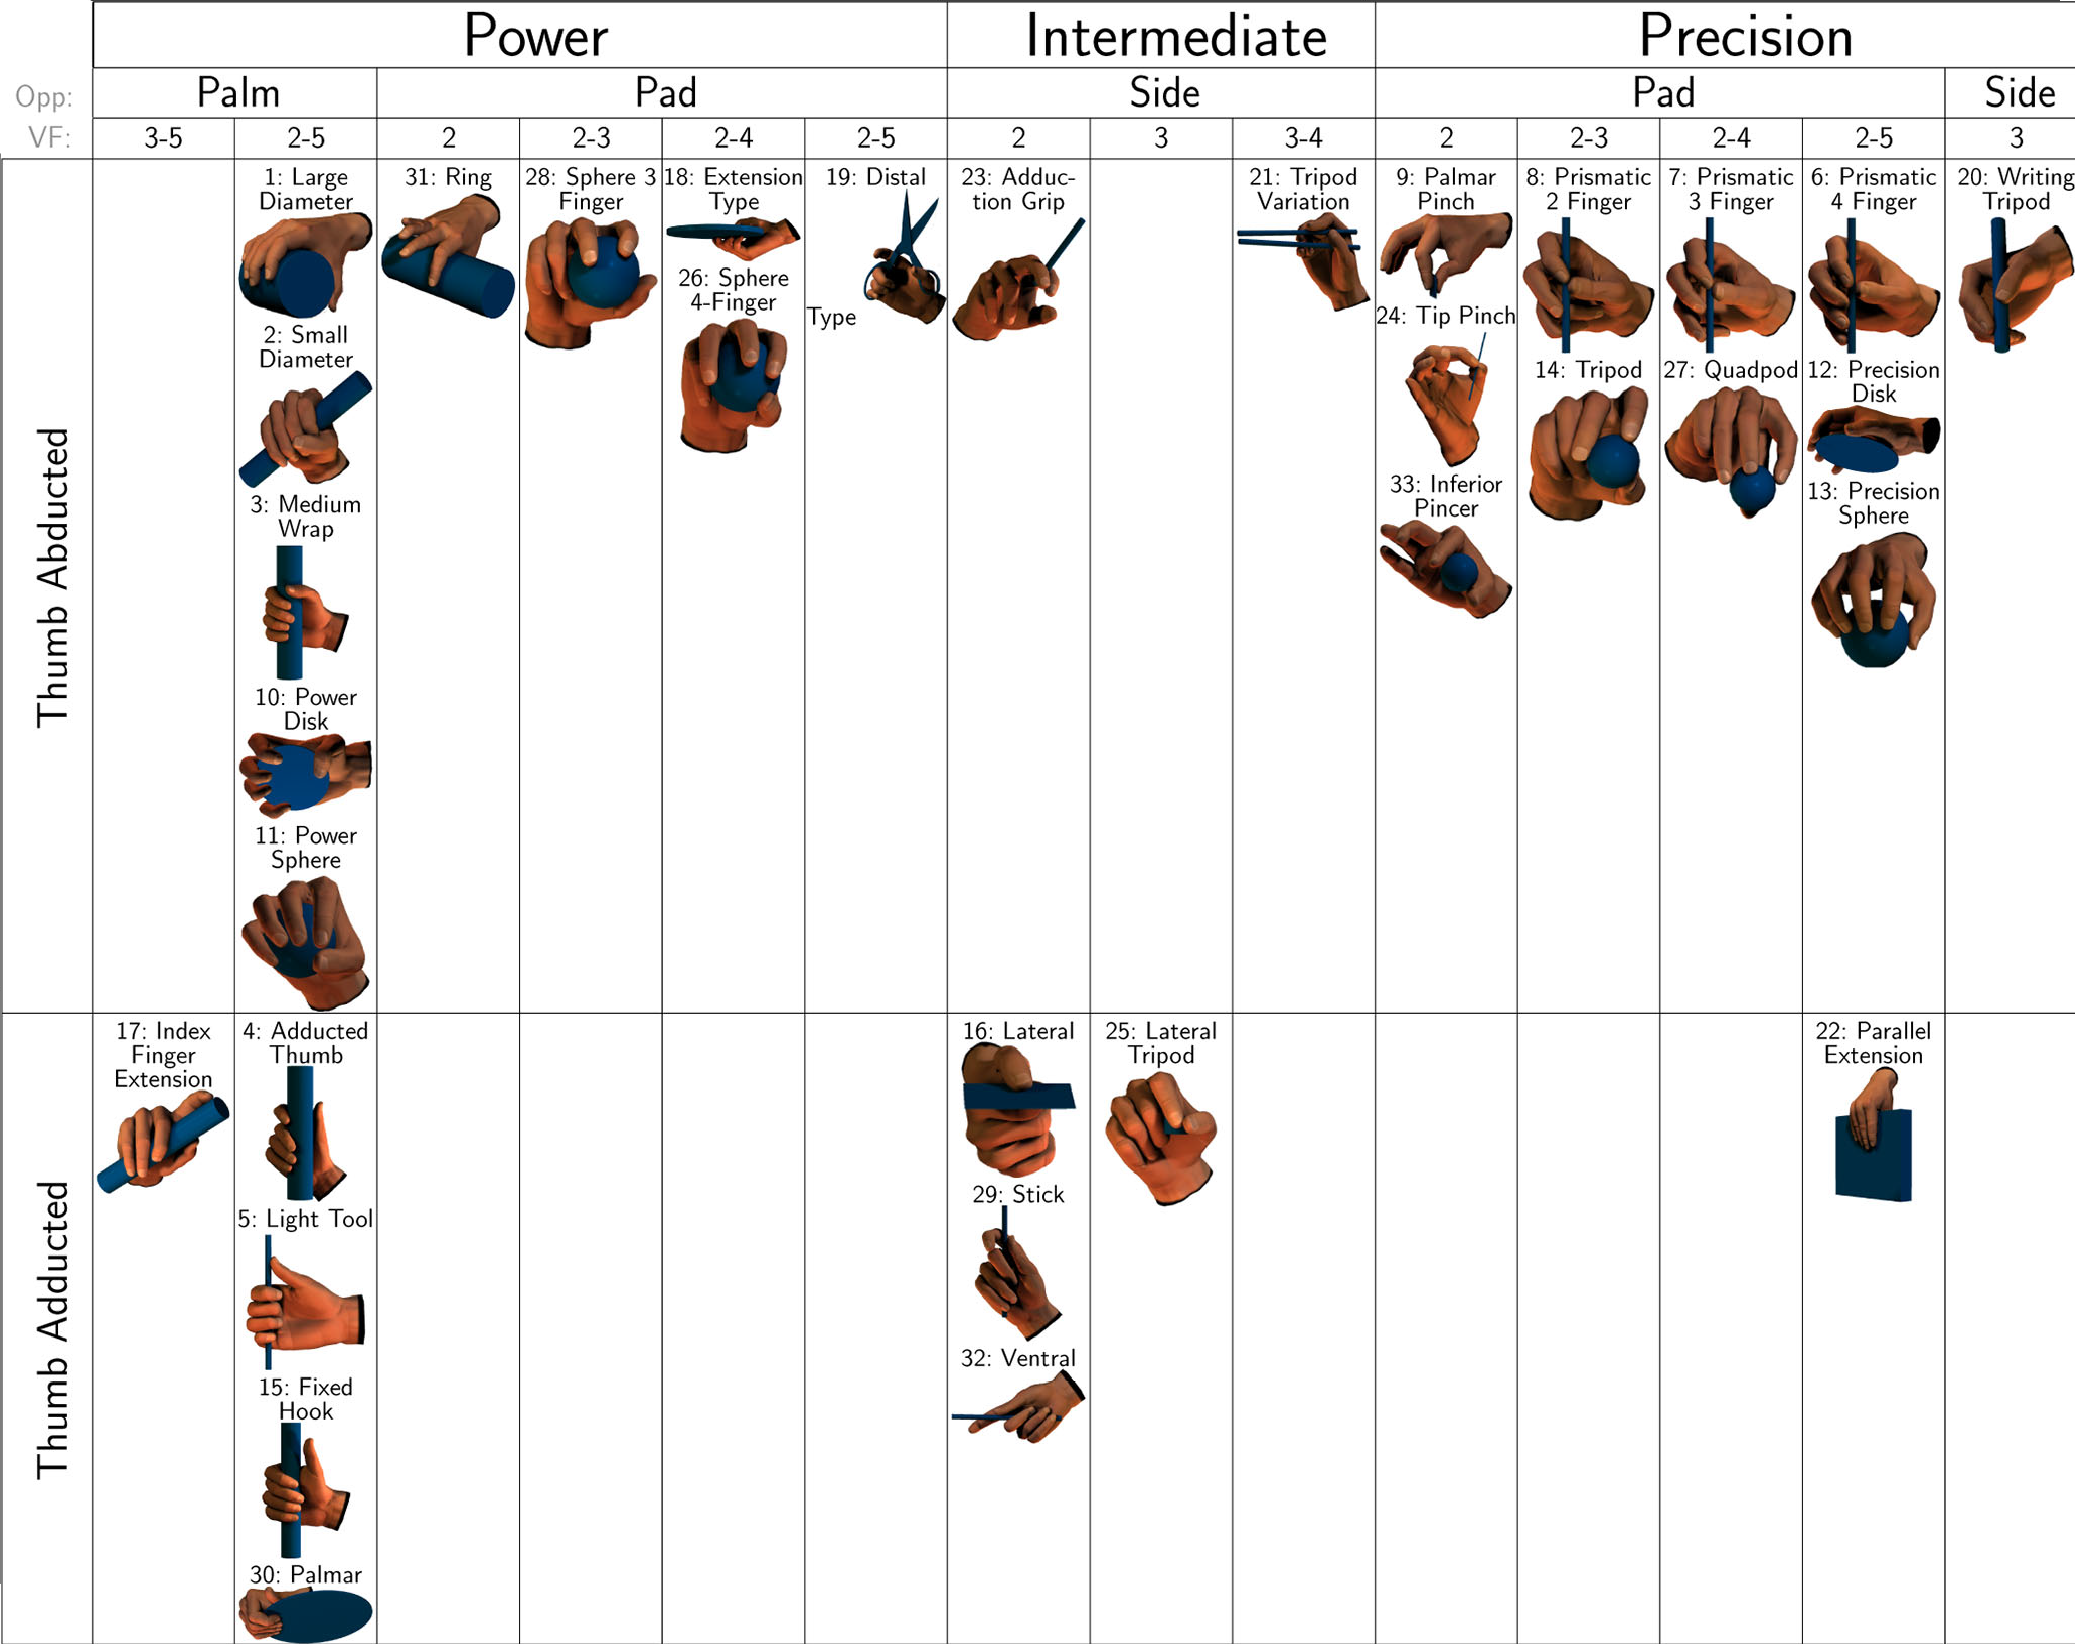
\includegraphics[width=0.60\linewidth]{imagens/agarres.PNG}
        \caption{Taxonom\'ia GRASP de tipos de agarre humano \cite{Feix2016}}
        \label{fig:agarres}
    \end{figure}
\end{frame}

%================================================%
% SECCION 2: Objetivo General
%================================================%
\section{Objetivo General}

\begin{frame}{Objetivo General}
    \small
    \begin{block}{Objetivo}
        Dise\~nar y construir un exoesqueleto de eslabones r\'igidos para realizar agarres de pinza fina, empleando t\'ecnicas de an\'alisis cinem\'atico y de optimizaci\'on para adaptar los par\'ametros del mecanismo a distintas medidas antropom\'etricas de la poblaci\'on mexicana.
    \end{block}
\end{frame}

%================================================%
% SECCION 3: Trabajo Anterior
%================================================%
\section{Trabajo Anterior}

\begin{frame}{Modelo CAD}
    \scriptsize
    Se muestra el modelo CAD completo con los tres mecanismos ensamblados, motores y sistemas de transmisi\'on incluidos (v\'ease Figura \ref{fig:vistas}).

    \vspace{-0.2cm}
    \begin{figure}
        \centering
        \begin{subfigure}[b]{0.24\textwidth}
            \centering
            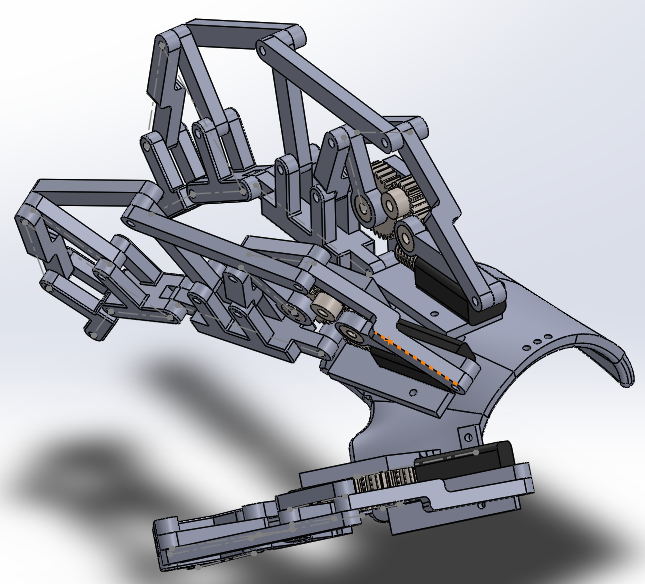
\includegraphics[width=\linewidth]{imagens/vista_iso.png}
            \caption{\tiny Isom\'etrico}
        \end{subfigure}
        \hfill
        \begin{subfigure}[b]{0.24\textwidth}
            \centering
            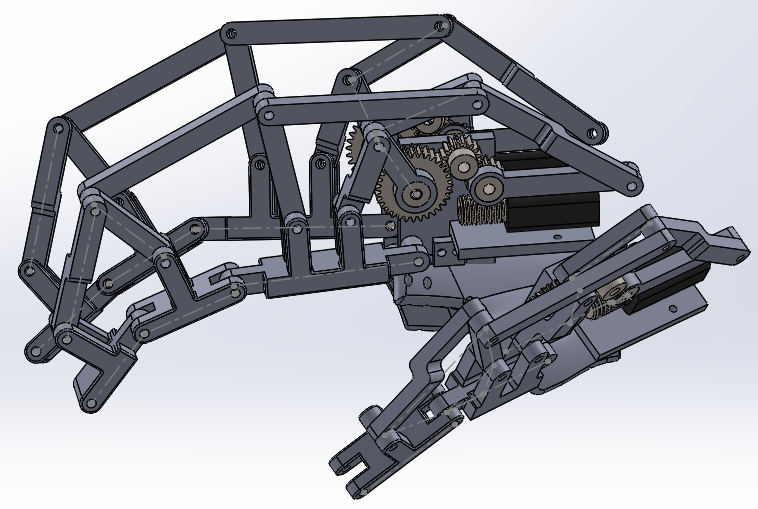
\includegraphics[width=\linewidth]{imagens/lateral.png}
            \caption{\tiny Vista lateral}
        \end{subfigure}
        \hfill
        \begin{subfigure}[b]{0.24\textwidth}
            \centering
            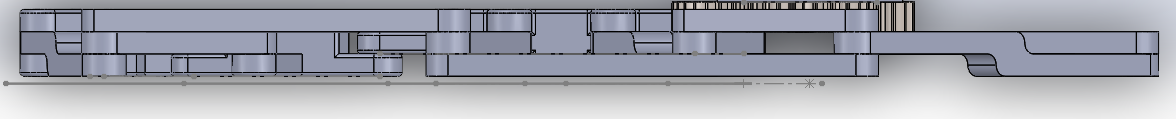
\includegraphics[width=\linewidth]{imagens/vista superior.png}
            \caption{\tiny Vista superior}
        \end{subfigure}
        \hfill
        \begin{subfigure}[b]{0.24\textwidth}
            \centering
            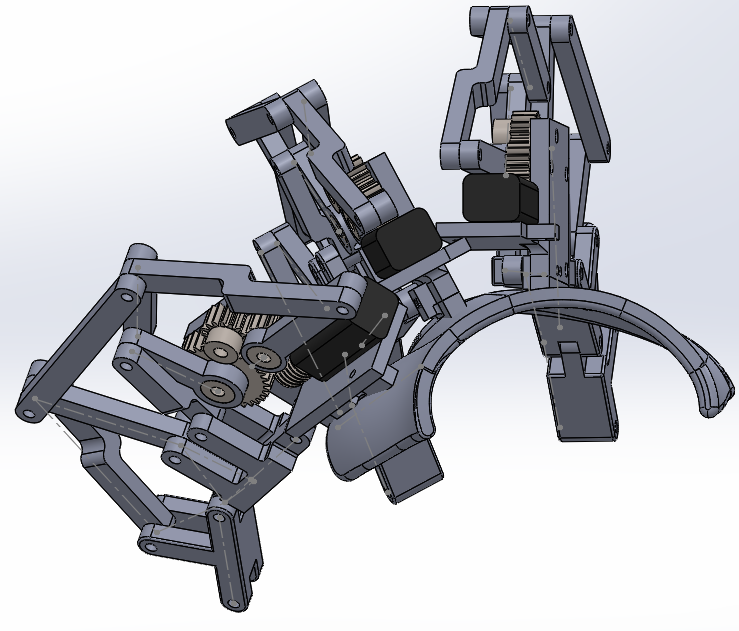
\includegraphics[width=\linewidth]{imagens/posterior.png}
            \caption{\tiny Vista posterior}
        \end{subfigure}

        \caption{Vistas del Modelo CAD}
        \label{fig:vistas}
    \end{figure}
\end{frame}

\begin{frame}{Construcci\'on}
    \begin{columns}[T]
        \begin{column}{0.50\textwidth}
            \small
            Una vez terminado el ensamble del modelo CAD, se procede con la construcci\'on de los mecanismos para cada dedo y la verificaci\'on del correcto movimiento (v\'ease Figura \ref{fig:mecanismo}).

            \vspace{0.3cm}
            Para las piezas se ha usado \textbf{impresi\'on 3D}.
        \end{column}

        \begin{column}{0.50\textwidth}
            \begin{figure}
                \centering
                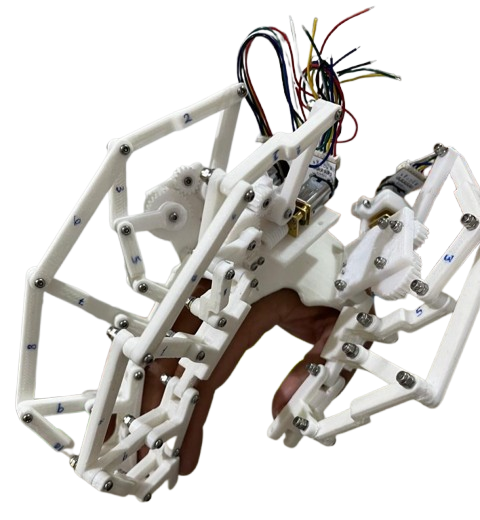
\includegraphics[width=0.95\linewidth]{imagens/isometrico_sf.png}
                \caption{Mecanismo construido}
                \label{fig:mecanismo}
            \end{figure}
        \end{column}
    \end{columns}
\end{frame}

\begin{frame}{Selecci\'on de Componentes}
    \small
    Se seleccionaron componentes mec\'anicos de transmisi\'on (m\'odulo $m=0.5$, metal) y un motor adecuado mediante una \textbf{matriz de decisi\'on ponderada}.

    \vspace{0.3cm}
    \textbf{Componentes principales:}
    \begin{itemize}
        \item \textbf{Motor:} Micro-reductor Pololu N20, 39 RPM, 6.7 kgf$\cdot$cm \cite{pololu_5202}
        \item \textbf{Engranes:} Par de engranes met\'alicos 15T/30T (reducci\'on 2:1)
        \item \textbf{Tornillo sin fin--corona:} Transmisi\'on a 90$^\circ$, reducci\'on elevada
        \item \textbf{Pi\~n\'on--cremallera:} Conversi\'on de movimiento rotacional a lineal (abducci\'on del pulgar)
    \end{itemize}

    \vspace{0.2cm}
    \begin{block}{Criterio de selecci\'on del motor}
        Evaluaci\'on ponderada: torque (20\%), velocidad (20\%), tama\~no (20\%), costo (10\%), \'angulo de giro (10\%), peso (10\%), voltaje (10\%). \textbf{Resultado: Pololu N20 (4.0/5.0)}.
    \end{block}
\end{frame}

%================================================%
% SECCION 4: Base de Datos
%================================================%
\section{Base de Datos}

\begin{frame}{Base de Datos}
    \small
    \textbf{Dataset de Pizzolato et al.} \cite{Pizzolato2017}
    \begin{itemize}
        \item Base de datos calibrada de movimientos y agarres de la mano.
        \item \textbf{40 sujetos} realizando diferentes tipos de agarres.
        \item Datos de cinem\'atica articular y electromiograf\'ia (EMG).
        \item Captura mediante sensores de movimiento (CyberGlove + marcadores \'opticos).
    \end{itemize}

    \vspace{0.3cm}
    \begin{block}{Aplicaci\'on en este proyecto}
        Se extraen las trayectorias articulares del dedo \'indice durante un agarre de pinza fina (125$^\circ$) para usarlas como \textbf{referencia en la optimizaci\'on} del mecanismo.
    \end{block}
\end{frame}

\begin{frame}{Selecci\'on del Agarre de Referencia}
    \small
    \textbf{Agarre seleccionado:} Pinza fina (125$^\circ$ de flexi\'on total)

    \vspace{0.2cm}
    \textbf{Articulaciones del dedo \'indice analizadas:}
    \begin{itemize}
        \item \textbf{IFP} (Interfal\'angica Proximal / PIP): uni\'on entre falange proximal y media.
        \item \textbf{IFD} (Interfal\'angica Distal / DIP): uni\'on entre falange media y distal.
        \item \textbf{TIP} (Punta del dedo): extremo de la falange distal.
    \end{itemize}

    \vspace{0.2cm}
    \textbf{Medidas antropom\'etricas utilizadas:}
    \begin{itemize}
        \item Falange proximal: 49 mm
        \item Falange media: 26 mm
        \item Falange distal: 24 mm
    \end{itemize}
\end{frame}

\begin{frame}{Trayectorias Articulares de Referencia}
    \scriptsize
    A partir de los \'angulos articulares de la base de datos (MCP, PIP y DIP) y las longitudes de las falanges (proximal: 49\,mm, media: 26\,mm, distal: 24\,mm), se calcul\'o la cinem\'atica directa del dedo para obtener las posiciones $(x, y)$ de cada articulaci\'on durante el agarre de pinza fina (0$^\circ$ a 125$^\circ$). Las trayectorias resultantes sirven como \textbf{referencia objetivo} para la optimizaci\'on del mecanismo (v\'ease Figura \ref{fig:tray_art}).

    \begin{figure}
        \centering
        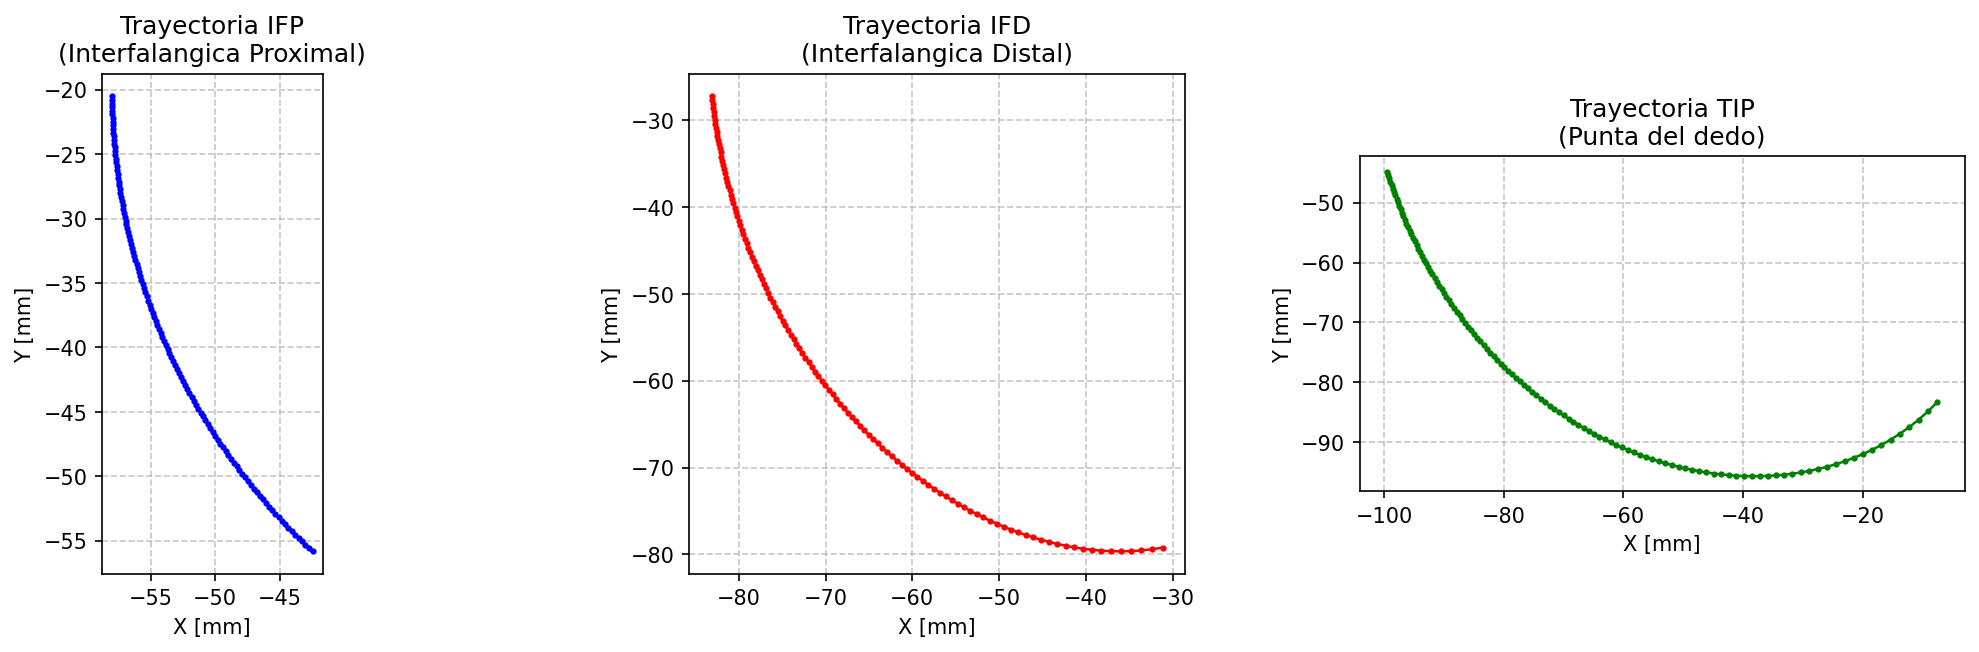
\includegraphics[width=0.90\linewidth]{imagens/trayectorias_articulares.png}
        \caption{Trayectorias articulares IFP, IFD y TIP del dedo \'indice}
        \label{fig:tray_art}
    \end{figure}
\end{frame}

%================================================%
% SECCION 5: Algoritmos de Optimizacion
%================================================%
\section{Algoritmos de Optimizaci\'on}

\begin{frame}{Motivaci\'on: Dise\~no de Trayectorias Bio-inspiradas}
    \begin{itemize}
        \item \textbf{Limitaci\'on Emp\'irica:} Los mecanismos dise\~nados por tanteo no logran reproducir la complejidad cinem\'atica natural del movimiento humano \cite{ebrahimi2015efficient}.
        \item \textbf{Acoplamiento Complejo:} El movimiento no es lineal; resulta de la interacci\'on coordinada entre m\'ultiples articulaciones \cite{Cabrera2002}.
    \end{itemize}

    \begin{block}{El Rol de la Optimizaci\'on}
        Permite ajustar las dimensiones geom\'etricas del mecanismo para \textbf{minimizar el error} entre la trayectoria anat\'omica real y la generada por el exoesqueleto \cite{deb2012optimization}.
    \end{block}

    \vspace{0.3cm}
    Se analizaron t\'ecnicas con cierta relevancia en s\'intesis de mecanismos y medicina de rehabilitaci\'on.
\end{frame}

%----------------------------------------------%
\begin{frame}{Algoritmos de Optimizaci\'on: M\'etodos Cl\'asicos}
\begin{table}
    \centering
    \tiny
    \renewcommand{\arraystretch}{1.2}
    \begin{tabularx}{\textwidth}{|>{\raggedright\arraybackslash}p{1.8cm}|X|X|X|}
        \hline
        \rowcolor[HTML]{C0C0C0}
        \textbf{T\'ecnica} & \textbf{Definici\'on} & \textbf{Ventajas} & \textbf{Desventajas} \\ \hline

        \textbf{Gradiente Descendente (GD)} & Minimiza iterativamente usando derivadas. Converge en direcci\'on opuesta al gradiente. & Simple, eficiente en funciones convexas. & No aplicable a funciones no diferenciables \cite{granada2006}. Alta probabilidad de convergencia local \cite{Rojas2018}. \\ \hline

        \textbf{Newton-Raphson (NR)} & Usa derivadas de 1er y 2do orden para hallar ra\'ices o puntos estacionarios. & Aplicable a optimizaci\'on no suave \cite{Loayza2024}. R\'apida convergencia cuadr\'atica. & C\'alculo del Hessiano costoso. Solo para funciones continuas \cite{Nocedal2006}. \\ \hline

        \textbf{Monte Carlo por Capas (MLMC)} & Simulaci\'on a lazo cerrado con valores aleatorios para minimizar el error total \cite{fernandez2019optimizacion}. & Alta precisi\'on con menor costo que el Monte Carlo cl\'asico. & Implementaci\'on compleja. Requiere modelo bien definido \cite{zhang2024computer}. \\ \hline
    \end{tabularx}
    \caption{Algoritmos de optimizaci\'on cl\'asicos}
    \label{tab:alg_opt}
\end{table}
\end{frame}

%-------------------------------------------------------%
\begin{frame}{Algoritmos de Optimizaci\'on: Metaheur\'isticas Bio-Inspirados}
\begin{table}
\centering
    \tiny
    \renewcommand{\arraystretch}{1.4}
    \begin{tabularx}{\textwidth}{|>{\raggedright\arraybackslash}p{2cm}|X|X|X|}
        \hline
        \rowcolor[HTML]{C0C0C0}
        \textbf{T\'ecnica} & \textbf{Definici\'on} & \textbf{Ventajas} & \textbf{Desventajas} \\ \hline

        \textbf{Algoritmos Gen\'eticos (GA)} & Simulan evoluci\'on natural (selecci\'on, cruce y mutaci\'on). & \'Util en espacios complejos. No requiere derivadas \cite{valencia1997optimizacion}. & Requiere calibraci\'on de par\'ametros \cite{zheng2024genetic}. \\ \hline

        \textbf{Enjambre de Part\'iculas (PSO)} & Imita el comportamiento colectivo de un enjambre. & Eficiente en problemas de alta complejidad \cite{lopez2014evaluacion}. F\'acil implementaci\'on. & Riesgo de estancarse en \'optimos locales \cite{zhang2015}. \\ \hline

        \textbf{Recocido Simulado (SA)} & Basado en el enfriamiento lento de metales para obtener estructuras resistentes \cite{abarca2015aplicaciones}. & Capacidad de escapar de \'optimos locales. & Lento, depende del esquema de enfriamiento \cite{centeno2016recocido}. \\ \hline

        \textbf{Colonia de Hormigas (ACO)} & Imita la b\'usqueda de rutas \'optimas mediante feromonas. & Efectivo en problemas de rutas y s\'intesis de mecanismos. & Alto costo computacional \cite{carlos2024}. \\ \hline

        \textbf{Evoluci\'on Diferencial (DE)} & Usa diferencias entre individuos para mutar soluciones. & Buena exploraci\'on en espacios continuos. & Sensible a la configuraci\'on de par\'ametros \cite{alonso2017}. \\ \hline
    \end{tabularx}
    \caption{\centering{Algoritmos de optimizaci\'on metaheur\'isticos, bio-inspirados}}
    \label{tab:alg_meta}
\end{table}
\end{frame}

%-------------------------------------------------------%
\subsection{Evaluaci\'on de las T\'ecnicas de Optimizaci\'on}

\begin{frame}{Comparativa Cualitativa de Algoritmos}
    \centering
    \small
    \renewcommand{\arraystretch}{1.2}
    \setlength{\tabcolsep}{5pt}

    \begin{table}
        \caption{An\'alisis Cualitativo de algoritmos}
        \label{tab:ana_cual}
        \begin{tabularx}{\textwidth}{|l|X|c|c|c|}
            \hline
            \rowcolor[HTML]{C0C0C0}
            \textbf{Algoritmo} & \textbf{Naturaleza} & \textbf{Explora.} & \textbf{Conver.} & \textbf{Robustez} \\ \hline
            \textbf{GD} & Gradiente & Muy Baja & R\'apida & Baja \\ \hline
            \textbf{NR} & Hessiano & Nula & Cuadr\'atica & Muy Baja \\ \hline
            \textbf{MLMC} & Muestreo & Media & Lenta & Alta \\ \hline
            \rowcolor[HTML]{E8F4FD}
            \textbf{GA} & Evolutivo & \textbf{Muy Alta} & Media & \textbf{Muy Alta} \\ \hline
            \textbf{PSO} & Enjambre & Alta & R\'apida & Media \\ \hline
            \textbf{SA} & T\'ermico & \textbf{Muy Alta} & Muy Lenta & Alta \\ \hline
            \rowcolor[HTML]{E8F4FD}
            \textbf{DE} & Diferencial & Alta & Med-R\'ap & \textbf{Muy Alta} \\ \hline
        \end{tabularx}
    \end{table}

    \vspace{0.2cm}
    \begin{itemize}
        \item \footnotesize \textbf{GA y DE} destacan por su alta robustez y capacidad de exploraci\'on en espacios de b\'usqueda complejos.
    \end{itemize}
\end{frame}

%-------------------------------------------------------%
\begin{frame}{An\'alisis Comparativo Cuantitativo de Algoritmos}
    \scriptsize
    \centering
    \renewcommand{\arraystretch}{1.2}
    \setlength{\tabcolsep}{2pt}

    \begin{tabularx}{\textwidth}{|X|c|c|c|c|>{\columncolor[HTML]{FFCE93}}c|c|c|c|}
        \hline
        \rowcolor[HTML]{C0C0C0}
        \textbf{Criterio de Evaluaci\'on} & \textbf{Peso} & \textbf{GD} & \textbf{NR} & \textbf{ML} & \textbf{GA} & \textbf{PSO} & \textbf{SA} & \textbf{DE} \\ \hline
        No dependencia de derivadas & 20\% & 1 & 1 & 5 & 5 & 5 & 5 & 5 \\ \hline
        Escape de m\'inimos locales & 25\% & 1 & 1 & 3 & 5 & 4 & 5 & 5 \\ \hline
        Manejo de restricciones (ROM) & 20\% & 2 & 1 & 4 & 4 & 4 & 3 & 4 \\ \hline
        Estabilidad num\'erica & 15\% & 4 & 2 & 4 & 4 & 5 & 4 & 5 \\ \hline
        Complejidad de implementaci\'on & 10\% & 5 & 4 & 3 & 5 & 5 & 4 & 4 \\ \hline
        Precisi\'on en trayectoria fina & 10\% & 3 & 5 & 2 & 5 & 4 & 3 & 4 \\ \hline
        \rowcolor[HTML]{EFEFEF}
        \textbf{Puntaje Total} & \textbf{100\%} & \textbf{2.1} & \textbf{2.0} & \textbf{3.6} & \textbf{4.65} & \textbf{4.4} & \textbf{4.2} & \textbf{4.6} \\ \hline
    \end{tabularx}

    \vspace{0.2cm}
    \footnotesize{Nota: Escala de 1 a 5.}
    \vspace{0.2cm}
    \begin{quote}
        \footnotesize
        \textbf{Resultado:} El \textbf{Algoritmo Gen\'etico (GA)} es seleccionado con un puntaje de \textbf{4.65}.
    \end{quote}
\end{frame}

%-------------------------------------------------------%
\begin{frame}{Selecci\'on del Algoritmo Gen\'etico}
    Algoritmos Gen\'eticos (GA) sobresale por su capacidad para optimizar sistemas complejos sin depender de derivadas \cite{deb2012optimization}. El algoritmo garantiza una exploraci\'on global que permite escapar de m\'inimos locales \cite{goldberg1989genetic}, asegurando el cumplimiento de las restricciones bio-mec\'anicas del usuario mediante un manejo de restricciones cinem\'aticas \cite{coello2002theoretical}.
\end{frame}


%================================================%
% SECCION 6: Optimizacion
%================================================%
\section{Optimizaci\'on}

\subsection{Modelo Cinem\'atico de Mecanismo de 4 Barras}
\begin{frame}{Modelo Cinem\'atico y S\'intesis de Trayectoria}
    \begin{columns}[T]
        \begin{column}{0.5\textwidth}
            \textbf{Configuraci\'on del Mecanismo:}
            \begin{itemize}
                \item Eslabones: $l_1$ (fijo), $l_2$ (manivela), $l_3$ (acoplador), $l_4$ (balanc\'in) \cite{Norton2012}.
                \item \textbf{Condici\'on de Grashof:} Para rotaci\'on continua:
                \[ s + l \leq p + q \]
                donde $s$ es el menor y $l$ el mayor.
            \end{itemize}
        \end{column}

        \begin{column}{0.5\textwidth}
            \textbf{Cierre de Lazo:}
            \begin{itemize}
                \item Verificaci\'on geom\'etrica:
                \[ |l_2 - l_3| \leq d \leq l_2 + l_3 \]
                \item Si no se cumple, el mecanismo es f\'isicamente imposible (soluci\'on descartada).
            \end{itemize}
        \end{column}
    \end{columns}

    \tiny
    \begin{block}{Trayectoria Objetivo}
        Se discretiza el movimiento de la falange distal ($N=50$ puntos):
        \[ x_{ref} = 0.05 \cos(\theta), \quad y_{ref} = 0.08 \sin(\theta) \]
        \textit{Intervalo de operaci\'on:} $\theta \in [0, \pi/2]$.
    \end{block}
\end{frame}

%-------------------------------------------%
\subsection{Algoritmo Gen\'etico: Par\'ametros y Funci\'on Fitness}
\begin{frame}{Optimizaci\'on mediante Algoritmo Gen\'etico (AG)}
    \small
    \textbf{Configuraci\'on del Vector de Dise\~no:}
    \centering $\mathbf{x} = [l_1, l_2, l_3, l_4]$ con $l_i \in [0.02, 0.15]\,m$.

    \begin{columns}[T]
        \begin{column}{0.45\textwidth}
            \textbf{Par\'ametros del AG:}
            \begin{itemize}
                \item \textbf{Poblaci\'on:} 120 individuos.
                \item \textbf{Generaciones:} 250.
                \item \textbf{Selecci\'on:} Torneo.
                \item \textbf{Cruce:} Aritm\'etico.
                \item \textbf{Mutaci\'on:} Perturbaci\'on aleatoria.
            \end{itemize}
        \end{column}

        \begin{column}{0.55\textwidth}
            \begin{exampleblock}{Funci\'on de Aptitud (Fitness)}
                Minimizaci\'on del Error Cuadr\'atico Medio (RMS):
                \[ E_{RMS} = \sqrt{\frac{1}{N} \sum_{i=1}^{N} \Delta P_i^2} \]
                donde $\Delta P_i$ es la distancia entre el punto generado y el de referencia.
            \end{exampleblock}
        \end{column}
    \end{columns}
\end{frame}

%-------------------------------------------%
\subsection{C\'odigo Python: Algoritmo Gen\'etico y Cinem\'atica}

\begin{frame}[fragile]{1era Versi\'on del Algoritmo de Optimizaci\'on}

\textbf{Trayectoria objetivo}

\begin{lstlisting}[language=Python,basicstyle=\ttfamily\tiny]
N = 50
theta_ref = np.linspace(0, np.pi/2, N)

x_ref = 0.05 * np.cos(theta_ref)
y_ref = 0.08 * np.sin(theta_ref)
\end{lstlisting}

\vspace{0.2cm}

\textbf{C\'alculo cinem\'atico}

\begin{lstlisting}[language=Python,basicstyle=\ttfamily\tiny]
Bx = l1 * np.cos(t)
By = l1 * np.sin(t)

Dx, Dy = l4, 0.0

d = np.sqrt((Bx - Dx)**2 + (By - Dy)**2)

cos_alpha = (l2**2 + d**2 - l3**2) / (2 * l2 * d)

alpha = np.arccos(cos_alpha)
beta = np.arctan2(By - Dy, Bx - Dx)

Cx = Bx + l2 * np.cos(beta + alpha)
Cy = By + l2 * np.sin(beta + alpha)
\end{lstlisting}

\vspace{0.2cm}

\textbf{Idea principal}
\scriptsize
\begin{itemize}
    \item Se genera la trayectoria del punto \(C\)
    \item Se eval\'ua si el mecanismo puede ensamblarse
    \item Se compara contra una trayectoria objetivo
\end{itemize}

\end{frame}

%---------------------------------------------------------------%

\begin{frame}[fragile]{Funci\'on Objetivo y Operadores Gen\'eticos}

\textbf{Funci\'on objetivo}

\begin{lstlisting}[language=Python,basicstyle=\ttfamily\tiny]
error = np.sqrt(np.mean(
    (x_mec - x_ref)**2 +
    (y_mec - y_ref)**2
))
\end{lstlisting}

\vspace{0.2cm}

\textbf{Cruce y mutaci\'on}

\begin{lstlisting}[language=Python,basicstyle=\ttfamily\tiny]
c1[i] = np.random.uniform(low, high)
c2[i] = np.random.uniform(low, high)

sigma = 0.01 * (1 - gen/max_gen)

ind = ind + np.random.normal(
    0, sigma, size=len(ind)
)
\end{lstlisting}

\vspace{0.2cm}

\textbf{Bucle principal}

\begin{lstlisting}[language=Python,basicstyle=\ttfamily\tiny]
for gen in range(generations):

    fitnesses = np.array([
        fitness(ind)
        for ind in population
    ])

    selected = tournament_selection(
        population, fitnesses
    )
\end{lstlisting}

\end{frame}

%--------------------------------------------%
\subsection{C\'odigo Python: M\'etodo de Procrustes}

\begin{frame}[fragile]{Ajuste geom\'etrico mediante Procrustes}
\scriptsize

\textbf{Problema detectado}

\vspace{0.2cm}

La trayectoria optimizada presentaba:

\begin{itemize}
    \item Ligera rotaci\'on
    \item Desplazamiento respecto a la trayectoria objetivo
\end{itemize}

\vspace{0.2cm}

Por ello se implement\'o un ajuste geom\'etrico basado en el m\'etodo de Procrustes.

\vspace{0.3cm}

\textbf{Centrado de trayectorias}

\begin{lstlisting}[language=Python,basicstyle=\ttfamily\tiny]
def center(x, y):

    return x - np.mean(x), \
           y - np.mean(y)
\end{lstlisting}

\vspace{0.2cm}

\textbf{Rotaci\'on de curvas}

\begin{lstlisting}[language=Python,basicstyle=\ttfamily\tiny]
def rotate_curve(x, y, theta):

    x_rot = x*np.cos(theta) - \
            y*np.sin(theta)

    y_rot = x*np.sin(theta) + \
            y*np.cos(theta)

    return x_rot, y_rot
\end{lstlisting}

\end{frame}

%---------------------------------------------------------------%

\begin{frame}[fragile]{C\'alculo de Rotaci\'on Optima y Error Alineado}

\textbf{\'Angulo \'optimo de alineaci\'on}

\begin{lstlisting}[language=Python,basicstyle=\ttfamily\tiny]
num = np.sum(
    x_ref * y_mec -
    y_ref * x_mec
)

den = np.sum(
    x_ref * x_mec +
    y_ref * y_mec
)

theta = np.arctan2(num, den)
\end{lstlisting}

\vspace{0.2cm}

\textbf{Error RMS alineado}

\begin{lstlisting}[language=Python,basicstyle=\ttfamily\tiny]
x_ref_r, y_ref_r = rotate_curve(
    x_ref, y_ref, theta
)

error = np.sqrt(np.mean(
    (x_ref_r - x_mec)**2 +
    (y_ref_r - y_mec)**2
))
\end{lstlisting}

\vspace{0.2cm}

\textbf{Integraci\'on en la funci\'on fitness}

\begin{lstlisting}[language=Python,basicstyle=\ttfamily\tiny]
return aligned_error(
    x_ref,
    y_ref,
    x_mec,
    y_mec
)
\end{lstlisting}

\end{frame}

%--------------------------------------------%
\subsection{Resultados: Trayectorias y Error (4 Barras)}

\begin{frame}{Trayectorias del Mecanismo de 4 Barras}
Resultado de la optimizaci\'on (Figura \ref{fig:tray_4b}).
    \begin{figure}
        \centering
        \begin{subfigure}[b]{0.48\textwidth}
            \centering
            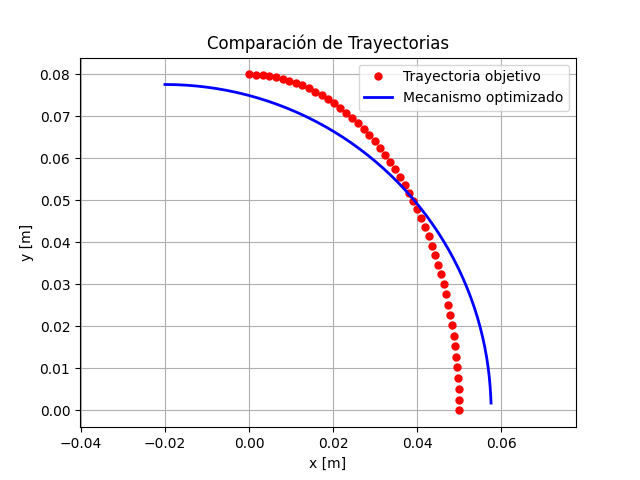
\includegraphics[width=\textwidth]{imagens/tray_opt2_sp.png}
            \label{fig:sin_procrustes}
        \end{subfigure}
        \hfill
        \begin{subfigure}[b]{0.48\textwidth}
            \centering
            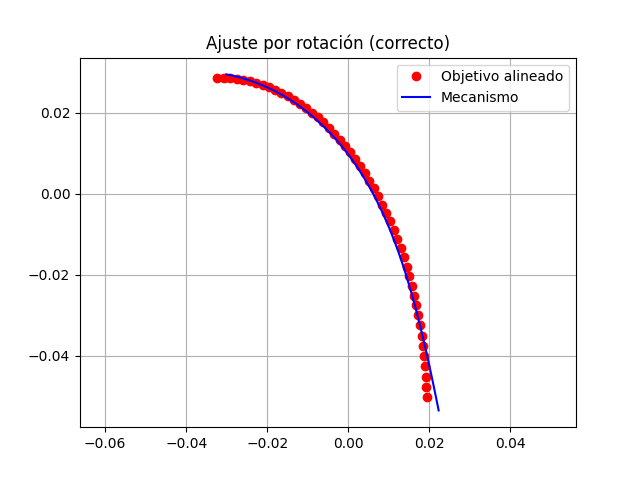
\includegraphics[width=\textwidth]{imagens/tray_opt3_cp.png}
            \label{fig:con_procrustes}
        \end{subfigure}

        \vspace{0.3cm}
        \caption{Trayectoria sin Procrustes vs. Usando Procrustes}
        \label{fig:tray_4b}
    \end{figure}
\end{frame}

%---------------------------------------------%
\begin{frame}{Error del Mecanismo de 4 Barras}
    \begin{itemize}
        \item Aunque la forma sea similar, el error RMS es alto debido a una notable rotaci\'on y ligero desplazamiento. El error se reduce al m\'inimo al implementar Procrustes (Figura \ref{fig:error_4b}).
    \end{itemize}
    \begin{figure}
        \centering
        \begin{subfigure}[b]{0.49\textwidth}
            \centering
            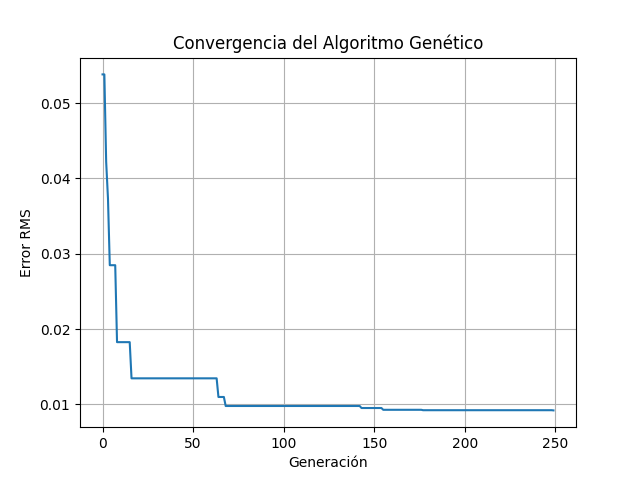
\includegraphics[width=\textwidth]{imagens/error_opt2_sp.png}
        \end{subfigure}
        \hfill
        \begin{subfigure}[b]{0.49\textwidth}
            \centering
            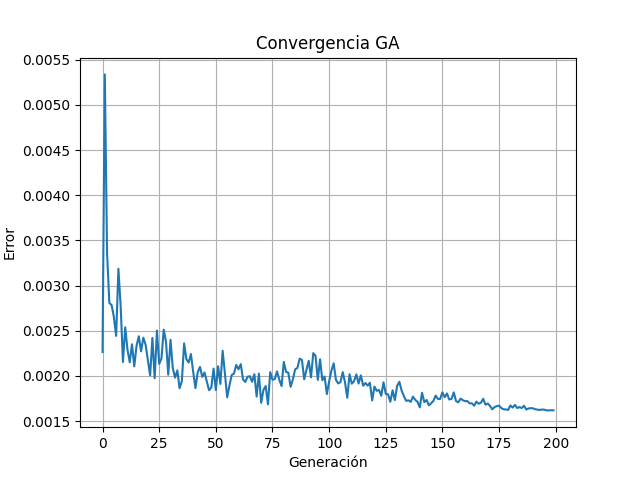
\includegraphics[width=\textwidth]{imagens/error_opt3_cp.png}
        \end{subfigure}

        \vspace{0.3cm}
        \caption{\centering Evoluci\'on del error sin Procrustes vs. Usando Procrustes}
        \label{fig:error_4b}
    \end{figure}
\end{frame}

%---------------------------------------------%
\begin{frame}{Validaci\'on del Mecanismo de 4 Barras}
\scriptsize
Se valida la optimizaci\'on mediante un simplificado modelo CAD.
     \vspace{-0.2cm}
     \begin{columns}[T]
        \begin{column}{0.5\textwidth}
            \begin{table}
                \centering
                \begin{tabular}{|c|c|}
                \hline
                \rowcolor[HTML]{C0C0C0}
                \textbf{Eslab\'on} & \textbf{Longitud}  \\ \hline
                  l1   &   7.0 cm \\ \hline
                  l2   &   2.0 cm \\ \hline
                  l3   &   7.2 cm \\ \hline
                  l4   &   2.0 cm \\ \hline
                \end{tabular}
                \caption{Longitudes \'optimas}
                \label{tab:longitudes_4b}
            \end{table}
        \end{column}

        \begin{column}{0.5\textwidth}
            \begin{figure}
                \centering
                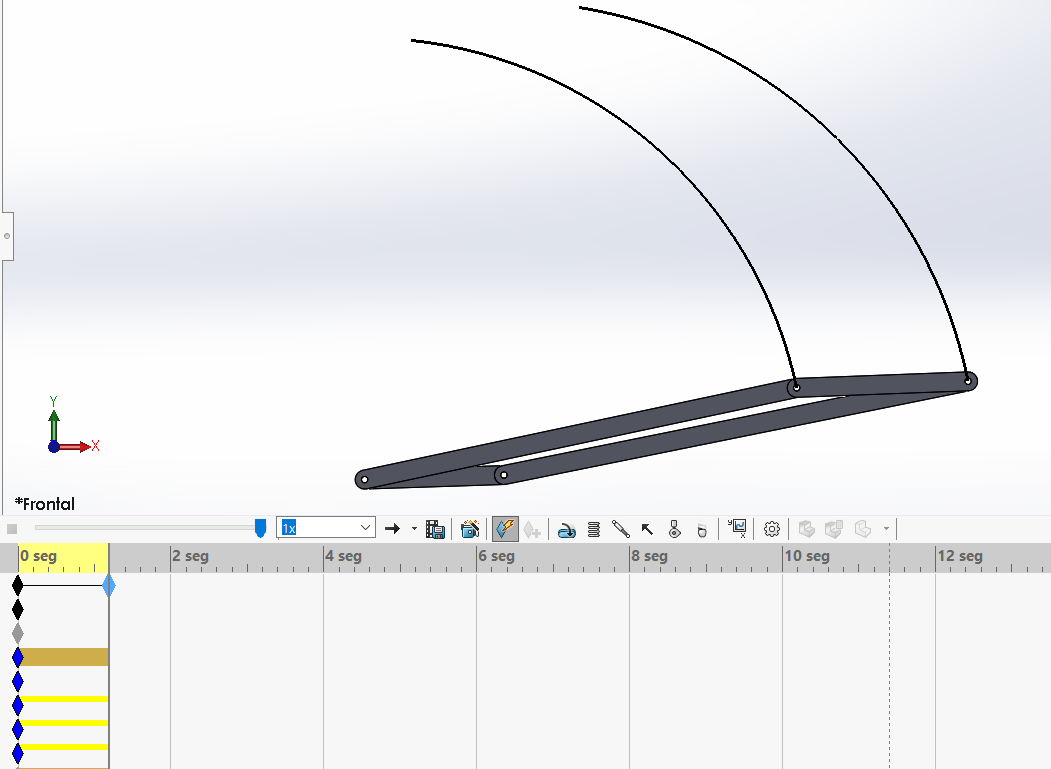
\includegraphics[width=0.85\linewidth]{imagens/estudio_mov.png}
                \caption{Mecanismo de 4 barras}
                \label{fig:mec_4b}
            \end{figure}
        \end{column}
    \end{columns}
\end{frame}

%---------------------------------------------%
\subsection{Mecanismo de 5 Barras: Topolog\'ia y Cinem\'atica}

\begin{frame}{Mecanismo de 5 Barras: Topolog\'ia y Cinem\'atica}
    \begin{columns}[T]
        \begin{column}{0.5\textwidth}
            \textbf{Configuraci\'on del Sistema:}
            \begin{itemize}
                \item \textbf{Eslabones:} $l_1, l_2$ (brazos actuados), $l_3, l_4$ (acopladores) y $l_5$ (base fija) \cite{Liu2006}.
                \item \textbf{Efector Final (P):} Punto de intersecci\'on entre $l_3$ y $l_4$.
                \item \textbf{Ventaja:} Mayor espacio de trabajo y versatilidad que el de 4 barras.
            \end{itemize}
        \end{column}

        \begin{column}{0.5\textwidth}
            \textbf{Modelo Cinem\'atico:}
            Se resuelve mediante la intersecci\'on de dos circunferencias con centros en las articulaciones m\'oviles $B$ y $D$:
            \begin{itemize}
                \item Circunferencia 1: $(x-B_x)^2 + (y-B_y)^2 = l_3^2$
                \item Circunferencia 2: $(x-D_x)^2 + (y-D_y)^2 = l_4^2$
            \end{itemize}
        \end{column}
    \end{columns}

    \scriptsize
    \begin{block}{Condici\'on de Existencia (Cierre Geom\'etrico)}
        Para que el mecanismo sea ensamblable, la distancia $d$ entre $B$ y $D$ debe cumplir:
        \[ |l_3 - l_4| \leq d \leq l_3 + l_4 \]
        \textit{Penalizaci\'on en c\'odigo:} $1 \times 10^4$ si la condici\'on se viola.
    \end{block}
\end{frame}

%--------------------------------------------------------%
\begin{frame}[fragile]{Modelo cinem\'atico del Mecanismo de 5 Barras}
\scriptsize
\textbf{Modelo cinem\'atico}

Se calcul\'o la posici\'on del efector final mediante
la intersecci\'on de dos circunferencias.

\vspace{0.1cm}

\begin{lstlisting}[language=Python,basicstyle=\ttfamily\tiny]
d = np.sqrt((Dx - Bx)**2 +
            (Dy - By)**2)

a = (l3**2 - l4**2 + d**2)/(2*d)

h = np.sqrt(l3**2 - a**2)

Px = Bx + a*(Dx - Bx)/d
Py = By + a*(Dy - By)/d

x = Px + h*(Dy - By)/d
y = Py - h*(Dx - Bx)/d
\end{lstlisting}

\textbf{Restricciones geom\'etricas}

\begin{lstlisting}[language=Python,basicstyle=\ttfamily\tiny]
if d > (l3 + l4):
    return None, None

if d < abs(l3 - l4):
    return None, None
\end{lstlisting}

\end{frame}

%------------------------------------------------%
\subsection{Resultados: Mecanismo de 5 Barras}

\begin{frame}{Resultados del Mecanismo de 5 Barras}

    \begin{itemize}
        \item Los mecanismos de 5 barras tienen mayor libertad geom\'etrica para trazar trayectorias \cite{ebrahimi2015efficient}.
        \item Longitudes \'optimas obtenidas: 5.48, 1.0, 1.01, 5.14, 1.0 cm.
        \item Restricciones de dise\~no: $0.01 \le l_i \le 0.07\;m$
    \end{itemize}

    \begin{figure}
        \centering
        \begin{subfigure}[b]{0.49\textwidth}
            \centering
            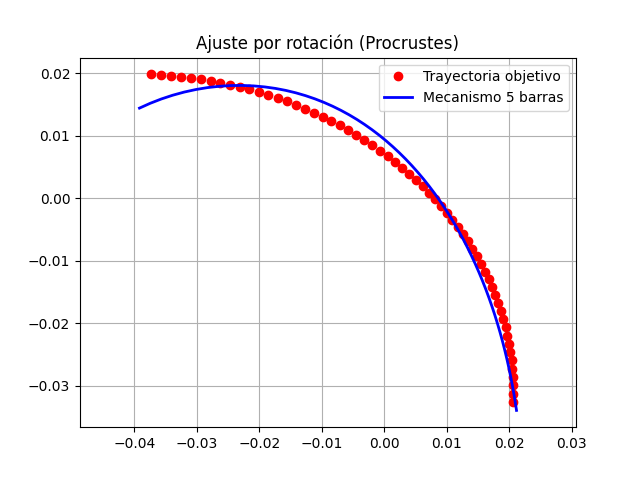
\includegraphics[width=\textwidth]{imagens/tray_5b.png}
        \end{subfigure}
        \hfill
        \begin{subfigure}[b]{0.49\textwidth}
            \centering
            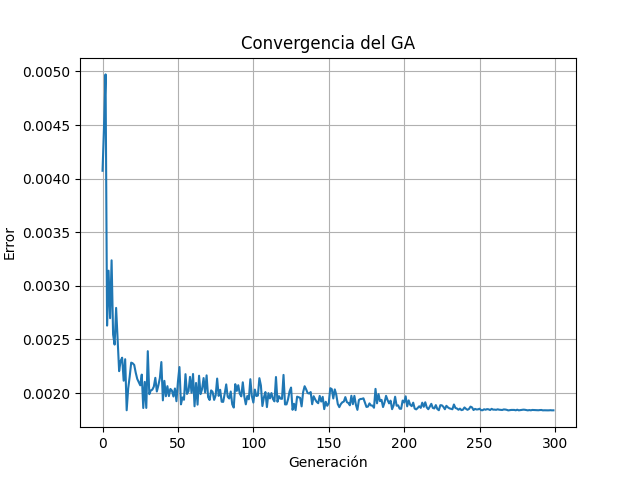
\includegraphics[width=\textwidth]{imagens/error_5b.png}
        \end{subfigure}

        \vspace{0.3cm}
        \caption{\centering Trayectoria y Evoluci\'on del Error - Mecanismo de 5 Barras}
        \label{fig:error_5b}
    \end{figure}
\end{frame}

%-------------------------------------------------------%
\subsection{Hiperheur\'istica + AG: Primer Intento}

\begin{frame}[fragile]{Hiperheur\'istica como Gestor del AG}
    \scriptsize
    \textbf{Idea:} Usar una hiperheur\'istica como seleccionador din\'amico entre operadores de cruce y mutaci\'on para optimizar el mecanismo completo (5 barras + 4 barras acoplados).

    \vspace{0.2cm}
    \textbf{Estructura del modelo:}
    \begin{itemize}
        \item Vector de dise\~no: 12 variables (bancadas, eslabones, falange, relaci\'on de engranes, offset angular).
        \item Modelo cinem\'atico: lazo de 5 barras $\rightarrow$ lazo de 4 barras $\rightarrow$ posici\'on IFP.
        \item Fitness: Error RMS + penalizaci\'on por compacidad.
    \end{itemize}

    \vspace{0.2cm}
    \textbf{Fragmento -- Hiperheur\'istica de mutaci\'on:}
\begin{lstlisting}[language=Python,basicstyle=\ttfamily\tiny]
def hyper_heuristic_mutation(ind):
    method = random.choice(['soft','aggressive'])
    if method == 'soft':
        idx = random.randint(0, len(ind)-1)
        ind[idx] += random.uniform(-0.005, 0.005)
    else:
        for i in range(len(ind)):
            if random.random() < 0.3:
                ind[i] += random.uniform(-0.02, 0.02)
    return ind
\end{lstlisting}
\end{frame}

%-------------------------------------------------------%
\begin{frame}{Resultados: Hiperheur\'istica + AG}
    \scriptsize
    \textbf{Par\'ametros:} Poblaci\'on: 60, Generaciones: 120, Mutaci\'on: 25\%, Cruce: 80\%.

    \textbf{Error RMS final: 0.006 m} (no satisfactorio).

    \begin{figure}
        \centering
        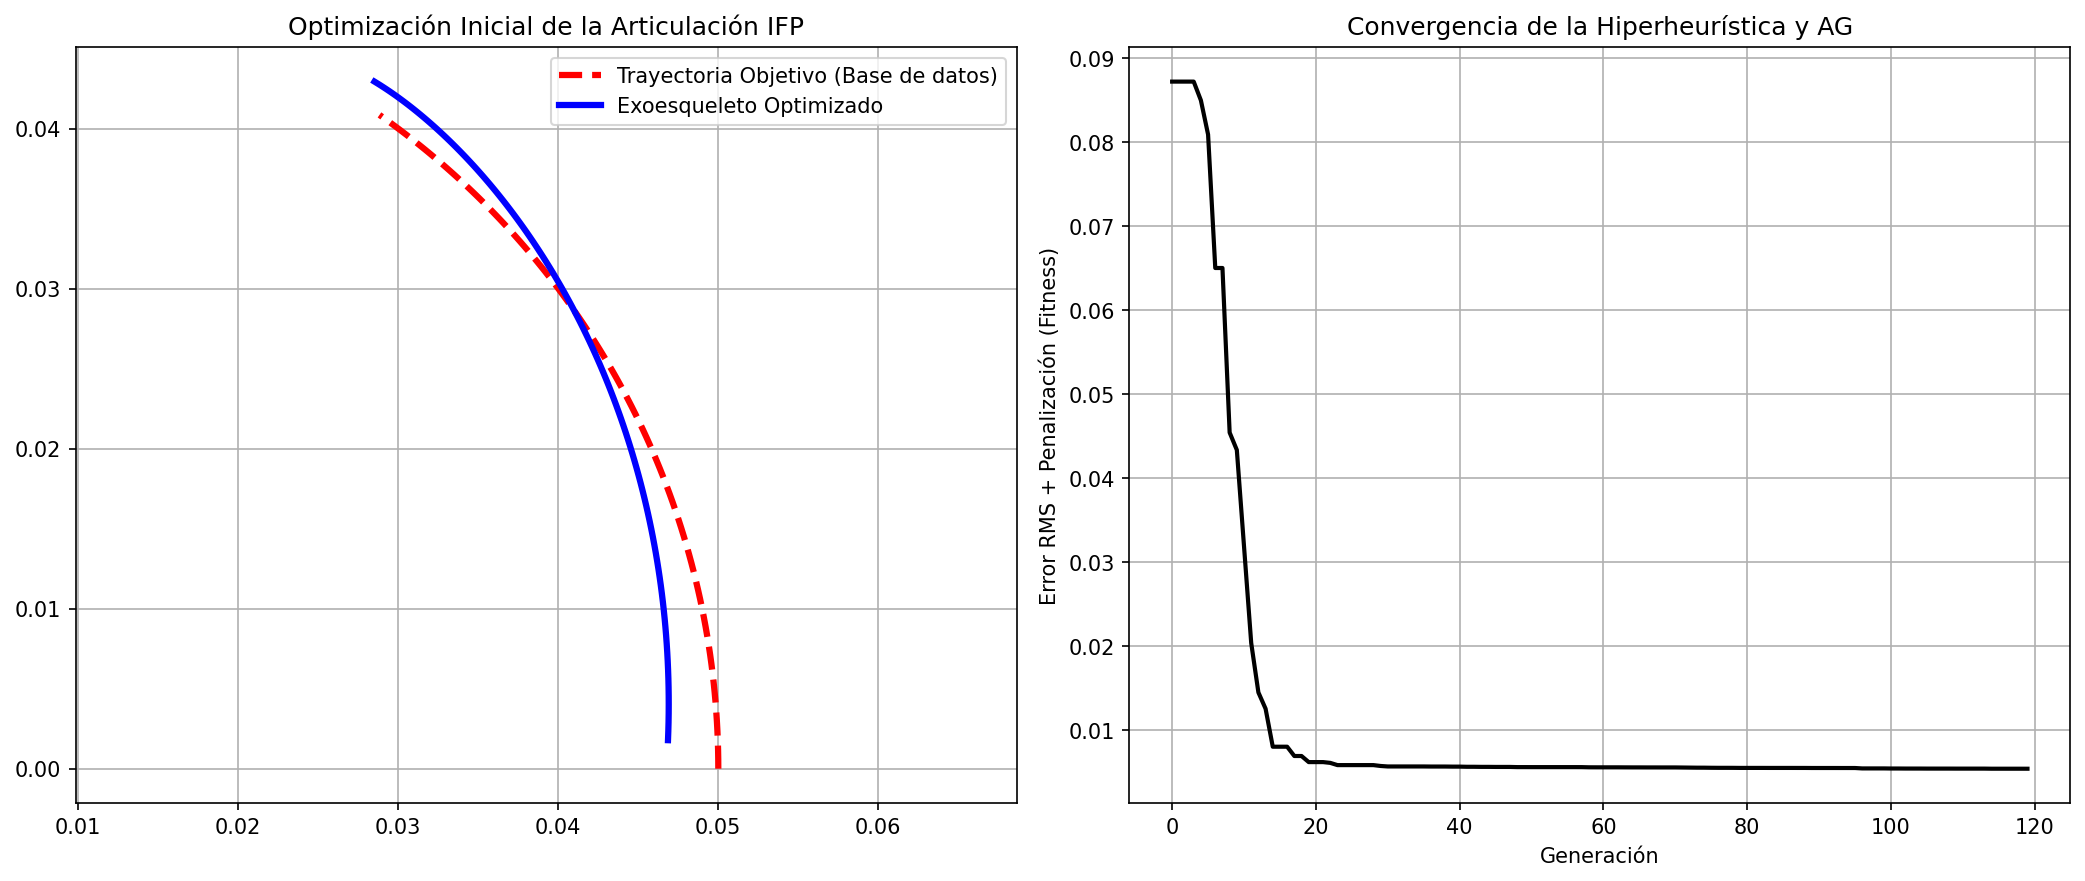
\includegraphics[width=0.85\linewidth]{imagens/resultado_hiper_AG.png}
        \caption{Resultado del AG con hiperheur\'istica para la articulaci\'on IFP}
        \label{fig:hiper_ag}
    \end{figure}

    \vspace{-0.2cm}
    \textbf{Problemas identificados:}
    \begin{enumerate}
        \item \textbf{Alta sensibilidad:} Las ecuaciones de cierre frecuentemente no tienen soluci\'on (penalizaci\'on $10^6$).
        \item \textbf{Hiperheur\'istica limitada:} Dificultad para mantener simult\'aneamente la trayectoria natural y las restricciones mec\'anicas.
        \item \textbf{Costo computacional:} Incremento excesivo al intentar reducir el error.
        \item \textbf{Longitudes no realistas:} Algunas longitudes de eslabones resultaron mayores a 10\,cm, excediendo las dimensiones f\'isicas del dedo.
    \end{enumerate}

    $\Rightarrow$ Se recurri\'o a \textbf{Evoluci\'on Diferencial (DE)} como alternativa.
\end{frame}

%================================================%
% SECCION 7: Conclusiones
%================================================%
\section{Conclusiones}

\begin{frame}{Conclusiones}
    \begin{itemize}
        \item Se implement\'o exitosamente un Algoritmo Gen\'etico para la optimizaci\'on de mecanismos de 4 y 5 barras.
        \item El m\'etodo de Procrustes mejor\'o significativamente la alineaci\'on entre trayectorias, reduciendo el error RMS.
        \item El mecanismo de 5 barras ofrece mayor flexibilidad geom\'etrica para reproducir trayectorias anat\'omicas.
        \item Los resultados obtenidos validan la viabilidad del enfoque de optimizaci\'on para el dise\~no del exoesqueleto.
        \item Se valid\'o el mecanismo de 4 barras mediante un modelo CAD simplificado.
    \end{itemize}
\end{frame}

%================================================%
% SECCION 8: Lo que falta
%================================================%
\section{Lo que falta}

\begin{frame}{Siguientes Pasos}
    \begin{itemize}
        \item Realizar la validaci\'on del algoritmo para el mecanismo de 5 barras.
        \item Implementar una hiperheur\'istica que act\'ue como un gestor inteligente del sistema completo. En lugar de ejecutar el Algoritmo Gen\'etico de forma est\'atica.
        \item Integrar los mecanismos optimizados al modelo CAD completo del exoesqueleto.
        \item Instrumentar el prototipo con actuadores y sensores.
        \item Realizar pruebas de funcionamiento con el prototipo f\'isico.
    \end{itemize}
\end{frame}

%================================================%
% SECCION 9: Cronograma de Actividades
%================================================%
\section{Cronograma de Actividades}

\begin{frame}{Cronograma}
    \begin{figure}
        \centering
        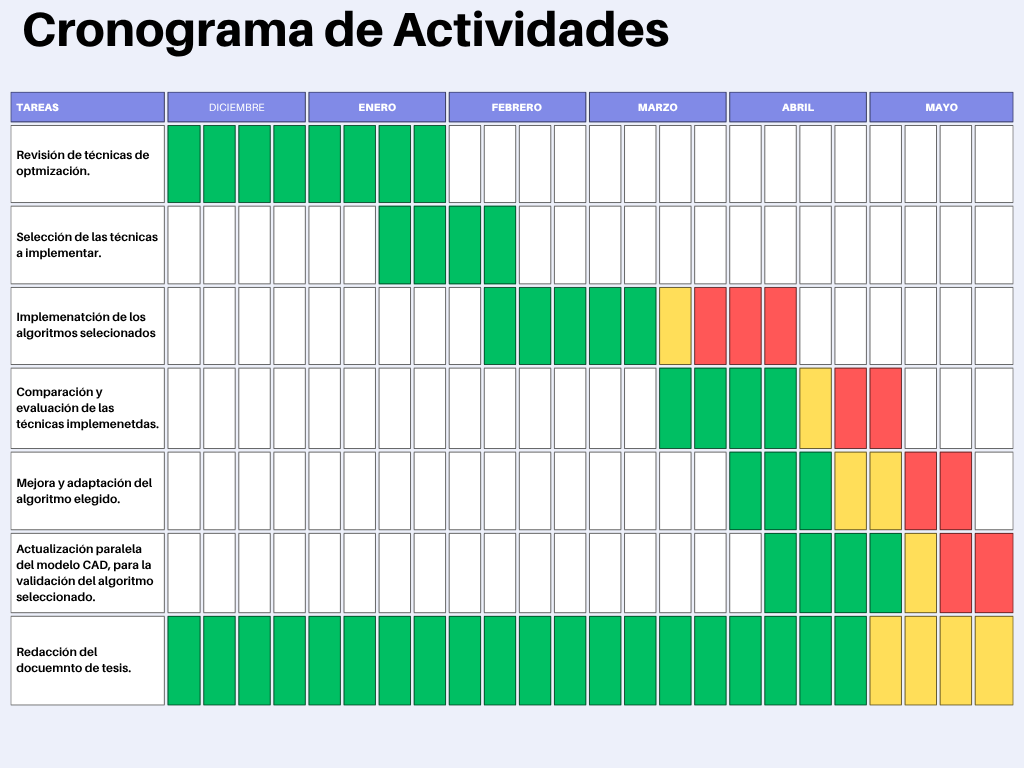
\includegraphics[width=0.95\linewidth]{imagens/2.png}
        \caption{Cronograma de actividades}
        \label{fig:crono}
    \end{figure}
\end{frame}

\begin{frame}{Actividad actual}
    \begin{figure}
        \centering
        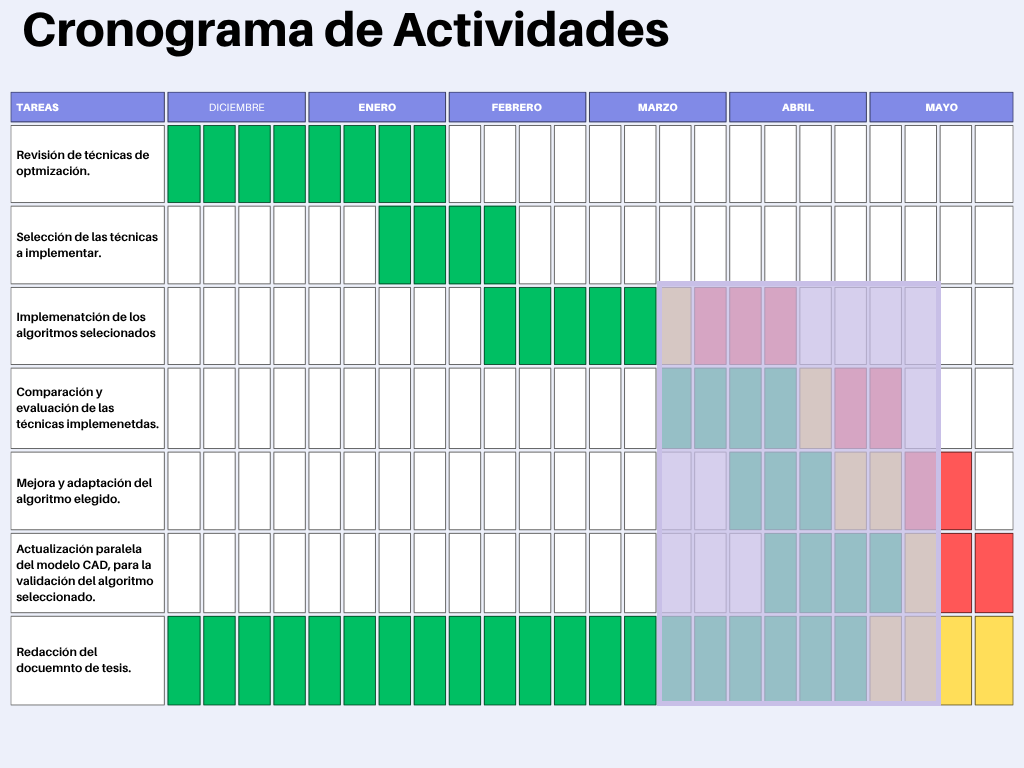
\includegraphics[width=0.95\linewidth]{imagens/2.1.png}
        \caption{Actividades actuales}
        \label{fig:crono2}
    \end{figure}
\end{frame}

%================================================%
% SECCION 10: Referencias
%================================================%
\section{Referencias}

\begin{frame}[allowframebreaks]{Bibliograf\'ia}
\bibliography{referencias}
\end{frame}

%================================================%
% SECCION 11: Gracias
%================================================%

\GraciasFrame

\end{document}
